\chapter{Bluetooth}
Bluetooth is a technology that allows for short-range wireless data transmission between two or more devices, developed as a wireless alternative to common cables. The Bluetooth technology was designed to emulate cables in costs, security and capabilities. \newline
Originally developed by Ericsson, Bluetooth technology is now used in millions of devices developed by many different manufacturers.
The development of the Bluetooth technology and the licensing of the trademark are now managed by the Special Interest Group, founded in 1998 by Ericsson, IBM, Intel, Nokia and Toshiba and now consisting of more than 25000 members.
Unlike Wi-Fi, Bluetooth is designed to be energy efficient and cheap to produce. For this reason, Bluetooth is very common on portable devices like smartphones and laptops.

\section{Overview}
Bluetooth devices operate in the ISM 2.4 Ghz band, a portion of the spectrum that can be utilized without licenses.
The spectrum, from 2400 to 2483.5 MHz, is partitioned in 79 radio channels.
The radio channels start at 2402 MHz and are 1 MHz wide.
Given that the ISM spectrum is utilized by many other technologies such as 802.11g/n, cordless phones and microwave ovens, Bluetooth has been designed to be noise tolerant. 
To achieve noise tolerance Bluetooth devices switch between the 79 available channels 1600 times per second in a pseudo-random fashion. This technique is called \emph{Channel Hopping}.
Two or more devices that have the same hopping pattern share a physical channel and are considered part of the same piconet.

\subsection{Piconets}
Piconets are the most basic form of Bluetooth communication upon which all other protocols are layered on.
In a piconet a device must act as a master and all the other devices as slaves.
The physical channel is divided into slots numbered according to the Bluetooth clock of the master.
A time division duplex scheme is used to schedule access to the channel and allow master and slaves to communicate.
All the communication in a piconet is between master and slaves, there is never direct communication between slaves.

\paragraph{Addressing}
Bluetooth radios, not unlike other network cards, are supplied by the manufacturer with a 48 bit long mac address.
This address is used to determine the hopping pattern of a device and to distinguish devices during the inquiry scan phase.
Devices participating in a piconet are addressed with a 3 bit long identifier which is only valid until they are active.
This means that only 7 slaves can concurrently participate in a piconet.
The master can keep track of inactive (parked) members of a piconet using a 8 bit long identifier.

\paragraph{Scatternets}
A device may be part of more than one piconet at the same time, but can only be the master of one. This kind of set-up is called a scatternet.
At a physical level this is achieved by time-sharing access to the Bluetooth radio.

\begin{figure}[h!]
  \centering
  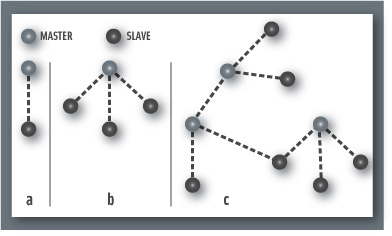
\includegraphics[width=0.7\textwidth]{img/piconets.jpg} 
  \caption{Piconets with a single slave operation (a), a multi-slave operation (b) and a scatternet operation (c).}
\end{figure}

\paragraph{Adaptive Frequency Hopping}
In a piconet the master may decide to alter the hopping sequence to only use a subset of the available 79 channels. The master will exclude  noisy channels and then communicate the new hopping pattern to all the slaves.

\subsection{Connection setup}
A connection is normally created following two steps: inquiry and page.
The inquiry scan is necessary to discover the mac addresses of devices that are in range and the paging procedure is used to establish the actual connection.
In the inquiry phase the source sends out inqury packets and then listens for inquiry reply.
If a listening device is in the inquiry phase it can receive and reply to such packets.
After the inquiry scan is complete a paging procedure can be started to establish the connection.
The device which starts the paging procedure will become master of the piconet formed as a result.

\subsection{Range}
Bluetooth divides devices into three classes based on how much transmission power they have, the transmission power influences the distance 

\vspace{0.3cm}
\begin{tabular}{|c|r|r|}
 \hline
 class & transmission power output & range \\ \hline
 1 & 100 mW & 100 meters \\
 2 & 2.5 mW & 10 meters \\
 3 & 1 mW & 1 meter \\
 \hline
\end{tabular}
\vspace{0.3cm} 

\noindent
Most modern smartphones are class 2 devices

\subsection{Baseband}
The \emph{baseband} implements the medium access control and physical layer parts of the Bluetooth system.
It manages physical channels and links, hop selection and scanning for nearby devices (inquiry scan).


\section{Bluetooth Architecture}
The Bluetooth technology is divided into two specifications: the core and the profile specifications. The core specification defines how the technology works, while the profiles define how to leverage on the core technologies to build a Bluetooth application.
The Bluetooth core system consists of an RF transceiver, the baseband, and a set of protocols.

\begin{figure}[ht!]
  \centering
  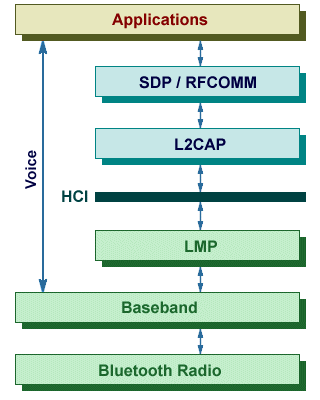
\includegraphics[width=0.3\textwidth]{img/bluetooth_protocol_stack.png} 
  \caption{Bluetooth protocol stack}
  \label{img:bt-protocol-stack}
\end{figure}

\subsection{L2CAP}
The L2CAP (Logical Link Control and Adaptation Layer) layer provides both connectionless and connection-oriented services to higher level protocols. Its tasks include multiplexing of protocols (since Baseband does not contemplate a "type" field to specify the kind of protocol that generated a package), segmentation and reassembly of PDUs (Protocol Data Unit), and QoS (Quality of Service) support.
L2CAP enables higher level applications and protocols to send and receive L2CAP data packets up to 64 kilobytes in length.

The L2CAP layer provides logical channels, named L2CAP channels, which act as a logical connection on top of a baseband connection.
More channels can rely on the same baseband connection.
An endpoint of an L2CAP channel is identified by a channel identifier (CID).

By default, L2CAP uses ACL as the transmission link.

\subsubsection{ACL}
Bluetooth supports two main types of connection links: ACL (Asynchronous Connection Less) and SCO (Synchronous Connection Oriented).
The most widely used one is ACL, which garantees that data is delivered and in the correct order and without errors.

ACL links can operate both in a symmetric and in a asymmetric mode, and can be granted a Quality of Service by setting the appropriate channel parameters during connection.

\subsection{RFCOMM}
The RFCOMM protocol emulates the capabilities of the RS-232 serial ports over the L2CAP protocol. It was developed to make it easier for manufacterers to use the Bluetooth technology in their existing applications. Similarly to TCP, RFCOMM provides applications a simple point-to-point reliable data stream, supporting multiplexing and flow control between devices and applications.

It is possible to maintain up to 60 simultaneous connections between two devices (each one can initialize up to 30 connections with the other one) using RFCOMM, while the maximum number of open simultaneous connections on a single device is implementation-specific.

Excluding Bluetooth LE (Low Energy), RFCOMM is the only Bluetooth protocol officially supported by the Android API.

\subsection{SDP}
The Service Discovery Protocol (SDP) enables Bluetooth devices to discover the existence and the attributes of services provided by other server applications.
SDP provides the ability for clients to search for needed services based on specific attributes of those services. 
However, it is possible to retrieve a list of all services with their attributes from another device.
This process is called browsing.

While SDP provides the means to discover services it does not provide a mechanism to utilize them.

SDP is bound to the L2CAP protocol.

\paragraph{Service Record}
All of the information about a service is stored by the SDP server as a single service record, which consists in a list of attributes.
Each attribute represent a characteristic of the service, such as the name or the UUID. Each attribute is stored as a ID-VALUE pair, where the ID is a 16 bit unsigned integer and the value is a variable length field.


\section{Bluetooth on Android}
Older versions of Android relied on BlueZ as the implementation of the Bluetooth stack.
Since version 4.2, BlueZ has been replaced by BlueDroid, an implementation of the Bluetooth Stack developed by Broadcom. 

The Android SDK only provides RFCOMM as the transport layer and wraps it into a Java Socket.